\section{Нелинейно-оптические процессы третьего порядка}\label{sec:nlin3}

\todo{пишем тут что нибудь? Может убрать деление на секции по статьям и оставить сквозную нумерацию в обзоре? для распространения импульсов в ОВ и мод это оправдано, так как используется и в ГВГ, и в ММЧВС}

\subsection{Распространение излучения в ОВ}
Распространение излучение в ОВ, как и в прочих средах, описывается уравнениями Максвелла~\cite{kalluri2013principles}. В СИ данные уравнения имеют вид:

\begin{subequations}\label{eq:maxwell}
	\begin{align}
		\nabla \times \mathbf{E} &= -\frac{\partial \mathbf{B}}{\partial t}, \\
		\nabla \times \mathbf{H} &= \mathbf{J} + \frac{\partial \mathbf{D}}{\partial t}, \\
		\nabla \cdot \mathbf{D} &= \rho_f, \\
		\nabla \cdot \mathbf{B} &= 0.
	\end{align}
\end{subequations}

В системе~\cref{eq:maxwell} величины $\mathbf{E}$ и $\mathbf{H}$~--- вектора напряжённости электрического и магнитного полей соответственно,  $\mathbf{D}$ и $\mathbf{B}$~--- соответствующие векторы электрической и магнитной индукции. Вектор плотности тока $\mathbf{J}$ и плотность свободных зарядов $\rho_f$ описывают источники электромагнитного поля. Если в среде отсутствуют свободные заряды, эти величины обращаются в нуль: $\mathbf{J}=\rho_f=0$.

Вектора индукции $\mathbf{D}$ и $\mathbf{B}$ возникают как отклик среды на распространение электрического и магнитного полей E и H. Связь между ними задаётся материальными уравнениями:

\begin{subequations}\label{eq:material}
	\begin{align}
		\mathbf{D} &= \epsilon_0 \mathbf{E} + \mathbf{P}, \\
		\mathbf{B} &= \mu_0 (\mathbf{H} + \mathbf{M}).
	\end{align}
\end{subequations}

В системе материальных уравнений~\cref{eq:material} $\epsilon_0$~--- электрическая постоянная, $\mu_0$~--- магнитная постоянная, $\mathbf{P}$ и $\mathbf{M}$~--- вектора индуцированной электрической и магнитной поляризации соответственно. Для немагнитной среды, такой как ОВ, $\mathbf{M} = 0$.

Исключая переменные $\mathbf{B}$ и $\mathbf{D}$ из \cref{eq:maxwell, eq:material}, находим связь между $\mathbf{E}$ и $\mathbf{H}$:

\begin{equation}
	\nabla \times \nabla \times \mathbf{E} = -\frac{1}{c^2} \frac{\partial^2 \mathbf{E}}{\partial t^2} - \mu_0 \frac{\partial^2 \mathbf{P}}{\partial t^2} \label{eq:wave}
\end{equation}

Здесь $c$~--- скорость света в вакууме, $\mu_0\epsilon_0 = 1/c^2$. Для решения волнового уравнения~\cref{eq:wave} необходима связь между поляризацией $\mathbf{P}$ и напряжённостью электрического поля $\mathbf{E}$. Ограничиваясь нелинейностями третьего порядка ($\chi^{(3)}$), индуцированную поляризацию можно представить в виде суммы линейного и нелинейного (по электрическому полю) слагаемых~\cite{boyd2008nonlinear}:

\begin{equation}
	\mathbf{P} = \varepsilon_0 \left( \chi^{(1)} \cdot \mathbf{E} + \chi^{(2)} : \mathbf{EE} + \chi^{(3)} \vdots \mathbf{EEE} + \ldots \right) = P_{\mathrm{L}} + P_{\mathrm{NL}}
	\label{eq:polarization}
\end{equation}

В~\cref{eq:polarization} предполагается мгновенный отклик среды, поэтому данное разложение не описывает эффекты, связанные с запаздыванием, такие как ВКР и ВРМБ. Восприимчивость первого порядка $\chi^{(1)}$ соответствует линейному отклику среды и определяет комплексный показатель преломления среды. Восприимчивость первого порядка $\chi^{(2)}$ отвечает за такие н-о эффекты, как ГВГ, ГСЧ, ГРЧ, оптическое выпрямление. В средах с отсутствием центра инверсии (таких как кварцевое стекло в ОВ) данная величина равна нулю. Однако, как будет показано в Главе~\cref{ch:nonlin2}, в ОВ возможна фотоиндуцированная запись решётки квадратичной нелинейности.
\subsection{Поперечные моды ОВ}\label{subsec:modes}

Рассмотрим волновое уравнение~\eqref{eq:wave} в отсутствие нелинейной поляризации ($\mathbf{P_{\mathrm{NL}}}=0$). Данное приближение допустимо, поскольку в кварцевых ОВ нелинейная восприимчивость третьего порядка $\chi^{(3)}$ много меньше линейной восприимчивости $\chi^{(1)}$, и при не слишком высоких напряжённостях электрического поля нелинейным вкладом в суммарную поляризацию~\eqref{eq:polarization} можно пренебречь. В этом случае поперечное распределение поля моды определяется исключительно линейным откликом среды. Переходя в частотное представление, запишем волновое уравнение в спектральном представлении:

\begin{equation}\label{eq:helmholtz_vector}
	\nabla \times \nabla \times \widetilde{\mathbf{E}}(\mathbf{r},\omega) = \varepsilon(\omega) \frac{\omega^2}{c^2} \widetilde{\mathbf{E}}(\mathbf{r},\omega)
\end{equation}

Воспользуемся соотношением из векторного анализа

\begin{equation}\label{eq:rotrot_identity_delta}
	\nabla \times \nabla \times \widetilde{\mathbf{E}} = \nabla(\nabla \cdot \widetilde{\mathbf{E}}) - \Delta \widetilde{\mathbf{E}},
\end{equation}

В~\cref{eq:rotrot_identity_delta} сравним порядки величин первого и второго слагаемых.

\begin{subequations}\label{eq:e0_estimation}
	\begin{align}
		\Delta \widetilde{\mathbf{E}} &\sim k_0^2E_0, \\
		\nabla(\nabla \cdot \widetilde{\mathbf{E}}) &= \nabla(-\nabla\epsilon \cdot \widetilde{\mathbf{E}}/\epsilon) \sim \nabla(\dfrac{\Delta\epsilon E_0}{a \epsilon}) \sim \dfrac{\Delta \epsilon}{a^2 \epsilon}
	\end{align}
\end{subequations}

В~\cref{eq:e0_estimation} $E_0$~--- характерная величина амплитуды поля, $\delta$~--- толщина переходного слоя на границе <<сердцевина-оболочка>>, $\Delta \varepsilon$~--- перепад диэлектрической проницаемости между сердцевиной и оболочкой. Пренебрежение первым слагаемым допустимо при выполнении условия:

\begin{equation}\label{eq:weak_guidance_criterion}
	\frac{\Delta \varepsilon}{\varepsilon} \cdot \frac{1}{(k_0 \delta)^2} \ll 1
\end{equation}

Для типичного ОВ ($\delta \approx 1~\text{мкм}$, $\lambda \approx 1~\text{мкм}$, $\Delta n/n \sim 10^{-3}$) отношение $\frac{\Delta\varepsilon}{\varepsilon} \frac{1}{(k_0 \delta)^2}$ не превышает $10^{-4}$, что позволяет пренебречь слагаемым $\nabla(\nabla \cdot \widetilde{\mathbf{E}})$ и перейти к уравнению Гельмгольца:

\begin{equation}\label{eq:helmholtz_n}
	\nabla^2 \widetilde{\mathbf{E}}(\mathbf{r},\omega) + n^2(\omega) \frac{\omega^2}{c^2} \widetilde{\mathbf{E}}(\mathbf{r},\omega) = 0
\end{equation}

где поглощение в среде считается пренебрежимо малым, вследствие чего показатель преломления $n(\omega)$ полагается чисто вещественной величиной.

\subsection{Четырёхволновое смешение}\label{subsec:fwm}
\subsubsection{Нелинейное волновое уравнение}

Четырёхволновое смешение (ЧВС) относится к параметрическим процессам третьего порядка, при которых три фотона передают свою энергию одному фотону на суммарной частоте либо два фотона аннигилируют с рождением двух новых фотонов при сохранении энергии и импульса \cite{agrawal2019} (см. схему на рис.~\cref{fig:fwm_principle}). Процесс с участием трёх фотонов, включающий в себя, в частности, генерацию третьей гармоники, требует выполнения крайне жёстких условий фазового синхронизма и в ОВ реализуется с низкой эффективностью, поэтому в дальнейшем рассматриваться не будет. В отличие от вынужденного рассеяния (ВКР или ВРМБ), где условие фазового синхронизма выполняется автоматически за счёт изменения свойств самой среды, при ЧВС необходимо целенаправленно обеспечивать фазовый синхронизм между взаимодействующими волнами путём выбора частот накачки и параметров волокна. Для вывода связанных уравнений, описывающих эволюцию комплексных амплитуд четырёх волн при ЧВС в оптическом волокне, принимаются следующие исходные положения:

\begin{figure}[htbp]
	\centering
	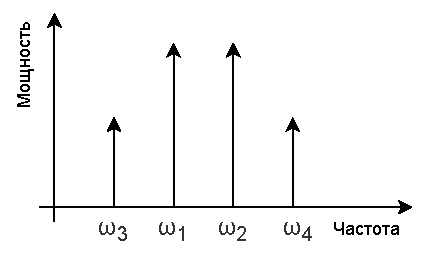
\includegraphics[width=0.4\linewidth]{Dissertation/images/review/fwm_principle}
	\caption{Принципиальная схема процесса ЧВС. Из закона сохранения энергии следует, что $\omega_1+\omega_2=\omega_3+\omega_4$}
	\label{fig:fwm_principle}
\end{figure}


\nomenclature{CW}{Сontinuous wave}
\nomenclature{QCW}{Quasi-continuous wave}


\begin{enumerate}
	\item Начинаем рассмотрение с волнового уравнения~\cref{eq:wave}, в котором нелинейная поляризация среды определяется откликом третьего порядка:
	\begin{equation*}
		\mathbf{P}_{\text{NL}} = \varepsilon_0 \chi^{(3)} \vdots \mathbf{EEE}
	\end{equation*}
	
	\item Рассматриваем скалярное приближение: все четыре взаимодействующие волны линейно поляризованы вдоль одной из осей, что обеспечивается использованием волокон с сохранением поляризации (например, типа PANDA)~\cite{fud3562,fud3564}. Данное приближение позволяет перейти от векторного описания к скалярному.
	
	\item Считаем излучение считается непрерывным (CW) или квазинепрерывным (QCW), что позволяет пренебречь зависимостью комплексных огибающих от времени. Данное приближение справедливо, если длительность оптического импульса значительно превышает как время нелинейного отклика среды (в кварцевом стекле составляет порядка нескольких фемтосекунд), так и масштаб дисперсионного уширения импульсов на длине волокна. В данной работе используются импульсы длительностью 2~нс, что удовлетворяет указанным критериям.
	
	\item Полагаем, что каждой спектральной компоненте соответствует своя поперечная мода ОВ, что учитывается при интегрировании по сечению и введении эффективной площади моды. Пространственная зависимость спектральных компонент представляется в виде
	\begin{equation*}
		E_j(\mathbf{r}) = F_j(x,y) A_j(z),
	\end{equation*}
	где $F_j(x,y)$~--- пространственное распределение $j$-й спектральной компоненты в поперечном сечении волокна.
\end{enumerate}


\begin{equation}
	\left\{\begin{array}{@{}l@{}}
		\dfrac{dA_1}{dz}=\dfrac{\im n_{nl} \omega_1}{c}\!\left[\left(f_{11}\left|A_1\right|^2+\sum\limits_{k\neq1}f_{1k}\left|A_k\right|^2\right)\!A_1+2f_{1234}A_2^{\ast}A_3A_4\e^{\im \Delta k z}\right]\!, \vspace{0.05cm} \\ 
		\dfrac{dA_2}{dz}=\dfrac{\im n_{nl} \omega_2}{c}\!\left[\left(f_{22}\left|A_2\right|^2+\sum\limits_{k\neq2}f_{2k}\left|A_k\right|^2\right)\!A_2+2f_{2134}A_1^{\ast}A_3A_4\e^{\im \Delta k z}\right], \vspace{0.05cm} \\
		\dfrac{dA_3}{dz}=\dfrac{\im n_{nl} \omega_3}{c}\!\left[\left(f_{33}\left|A_3\right|^2+\sum\limits_{k\neq3}f_{3k}\left|A_k\right|^2\right)\!A_3+2f_{3412}A_4^{\ast}A_2A_1\e^{-\im \Delta k z}\right], \vspace{0.05cm} \\
		\dfrac{dA_4}{dz}=\dfrac{\im n_{nl} \omega_4}{c}\!\left[\left(f_{44}\left|A_4\right|^2+\sum\limits_{k\neq4}f_{4k}\left|A_k\right|^2\right)\!A_4+2f_{4312}A_3^{\ast}A_2A_1\e^{-\im \Delta k z}\right].
	\end{array}\right.\,	
	\label{eq:mainEQfwm}
\end{equation}

Здесь $A_{{i}}$~--- амплитуды взаимодействующих волн с циклическими частотами $\omega_i$; $n_{nl}$~--- нелинейный показатель преломления; $f_{ij}\text{ и }f_{ijkl}$ $\left(i,j,k,l\in\left[1,\,4\right]\right)$~--- интегралы перекрытия между поперечными модами ОВ и их парами соответственно; $z$~--- продольная координата; $\Delta k$~--- волновая расстройка:


\begin{equation}
	\Delta k ={{n_3}\omega_3}/{c}+{{n_4}\omega_4}/{c}-{{n_1}\omega_1}/{c}-{{n_2}\omega_2}/{c}.
	\label{eq:deltaK}
\end{equation}

Здесь ${n_{i}}$~--- эффективный модовый показатель преломления, $c$~--- скорость света в вакууме.

Система уравнений~\cref{eq:mainEQfwm} допускает аналитическое решение в приближении неистощимой накачки. В рамках этого приближения амплитуды волн накачки считаются постоянными по длине волокна: \(|A_1(z)| \approx \mathrm{const}\) и \(|A_2(z)| \approx \mathrm{const}\).

Будем считать интегралы перекрытия приблизительно равными и обратно пропорциональными эффективной площади моды \(A_{\text{eff}}\):

\begin{equation}
	f_{ij} \approx f_{ijkl} \approx 1/A_{\text{eff}},\quad \left(i,j,k,l=1,2,3,4 \right),
	\label{eq:f_ij_ijkl_same}
\end{equation}

В этом случае эволюция сигнальной и холостой волн определяется величиной обобщённой фазовой расстройки $\kappa$:

\begin{equation}
	\kappa \coloneqq \Delta k  + \gamma\left(P_1 + P_2\right)
	\label{eq:nondepleted_phase_sync}
\end{equation}

где \(P_1 = |A_1|^2\) и \(P_2 = |A_2|^2\)~--- мощности волн накачки, \(\Delta k\) определяется выражением~\cref{eq:deltaK}, \(\gamma_i = n_2 \omega_i / (c A_{\text{eff}})\approx \gamma\).

При условии $\kappa=0$ зависимость мощности сигнальной и холостой волн от продольной координаты \(z\) становится экспоненциальной. Зависимость коэффициента усиления $g$ от величины обобщённой фазовой расстройки имеет вид:

\begin{equation}
	g=\sqrt{\left(2\gamma\sqrt{P_1 P_2}\right)^2-\left(\kappa/2\right)^2}
	\label{eq:gain_fwm}
\end{equation}

Оценки показывают~\cite{agrawal2019}, что коэффициент параметрического усиления при ЧВС превышает пиковое значение рамановского усиления примерно на $70\%$. Как следствие, при обеспечении условий фазового синхронизма порог возникновения ЧВС оказывается  ниже порога ВКР.

Взаимное влияние ЧВС и ВКР может приводить к интересным с научной точки зрения и полезным с практической точки зрения результатам. Так, в работе~\cite{eibl2017pulse} экспериментально продемонстрирована возможность создания трёхволнового лазерного источника на основе механизма комбинационного смещения с параметрической затравкой. В работе используется стандартное одномодовое волокно с положительной дисперией.  В такой среде условия фазового синхронизма для ЧВС не выполняются, и генерация новых спектральных компонент за счет только этого процесса была бы подавлена. Принципиальная схема установки приведена на рис.~\ref{fig:fewe_fwm}.
\nomenclature{MOPA}{Master Oscillator Fiber Amplifier}
\nomenclature{EOM}{Electro-Optic Modulator}
\nomenclature{YDFA}{Ytterbium Doped Fiber Amplifier}
\nomenclature{WDM}{Wavelength Division Multiplexer}
\nomenclature{OSA}{Optical Spectrum Analyzer}


\begin{figure}[htbp]
	\centering
	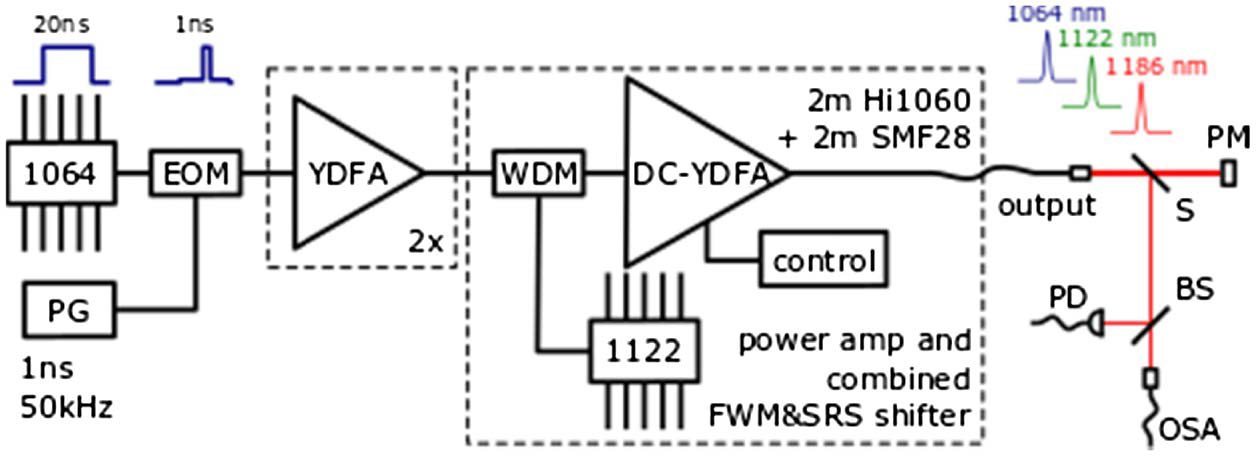
\includegraphics[width=0.6\linewidth]{Dissertation/images/review/fewe_scheme}
	\caption{Схема эксперимента. EOM~--- электрооптический модулятор; YDFA~--- иттербиевый волоконный усилитель; WDM~--- мультиплексор; OSA~--- оптический спектроанализатор.}
	\label{fig:fewe_scheme}
\end{figure}

Установка, изображённая на рис.~\cref{fig:fewe_scheme}, включает иттербиевый волоконный усилитель, работающий по MOPA-схеме и генерирующий импульсы накачки на $1064$~нм, а также задающий лазерный диод, обеспечивающий слабую затравочную волну на $1122$~нм, соответствующую первому стоксовому сдвигу.

При пиковой мощности накачки менее $1$~кВт на выходе преобладает излучение на длине волны $1064$~нм. С повышением мощности до величины около $1.3$~кВт вследствие развития эффекта ВКР усиливается и становится доминирующей спектральная компонента на $1122$~нм. При дальнейшем увеличении оптической мощности вступает в силу совместное действие каскадного ВКР и ЧВС, в котором волна $1122$~нм выступает в роли накачки, а волна $1186$~нм~--- в роли холостой компоненты. Поскольку её частота попадает в полосу стоксового усиления, повышение её мощности возможно даже в отсутствие фазового синхронизма для ЧВС. Высокий коэффициент усиления достигается за счет ВКР, а узкая спектральная линия формируется благодаря параметрической природе ЧВС-затравки. Описанная динамика переключения длин волн проиллюстрирована на рис.~\cref{fig:fewe_fwm}.

\begin{figure}[htbp]
	\centering
	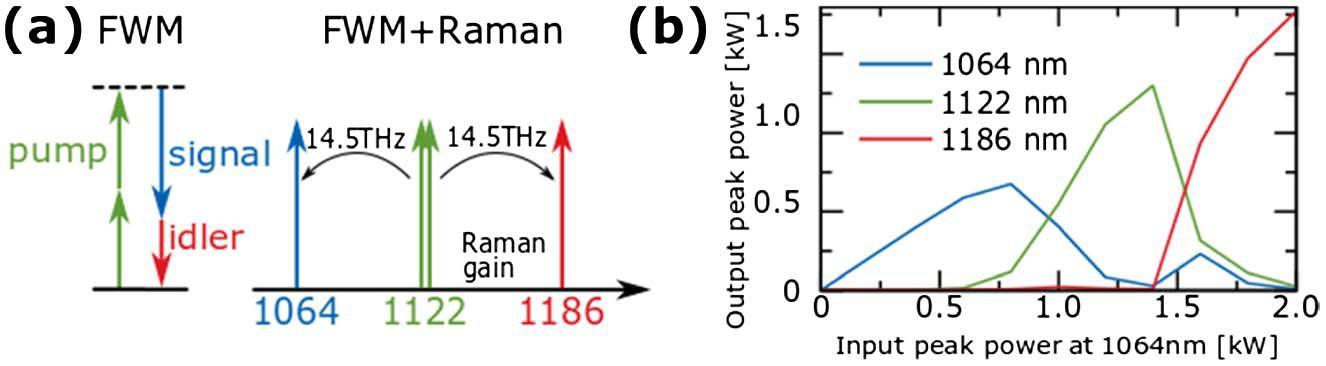
\includegraphics[width=0.7\linewidth]{Dissertation/images/review/fewe_fwm}
	\caption{(а) Совместное действие ЧВС и ВКР в ОВ приводит к генерации узкополосного излучения на $1186$~нм. (б) Результаты моделирования выходной мощности для трёх спектральных компонент ($1064$, $1122$ и $1186$~нм) при изменении мощности накачки на $1064$~нм и фиксированной мощности затравки на $1122$~нм}
	\label{fig:fewe_fwm}
\end{figure}

 Результаты данной работы показывают, что взаимное влияние двух н-о процессов могут приводить эффективной генерации новых спектральных компонент даже в отсутствие фазового синхронизма. Тем не менее, в практических применениях, когда эффект ВКР проявляется в меньшей степени, эффективность ЧВС критически зависит именно от выполнения условий фазового синхронизма. В связи с этим далее рассматриваются физические механизмы и практические методы его обеспечения.

\subsubsection{Фазовый синхронизм при ЧВС}
\subsubsection{Подавление ММЧВС}


\subsection{Методы математического моделирования н-о эффектов третьего порядка при распространении оптических импульсов по ОВ}